\documentclass{acmtog} % V1.2

\usepackage{hyperref}
\hypersetup{ colorlinks = true, linkcolor = black, urlcolor = blue, citecolor = blue }
\usepackage{float}
\let\oldquote\quote
\let\endoldquote\endquote
\renewenvironment{quote}[2][]
  {\if\relax\detokenize{#1}\relax
     \def\quoteauthor{#2}%
   \else
     \def\quoteauthor{#2~---~#1}%
   \fi
   \oldquote}
  {\par\nobreak\smallskip\hfill(\quoteauthor)%
   \endoldquote\addvspace{\bigskipamount}}

\acmVolume{1}
\acmNumber{1}
\acmYear{2018}
\acmMonth{March}
\acmArticleNum{1}
\makeatletter
\def\runningfoot{\def\@runningfoot{}}
\def\firstfoot{\def\@firstfoot{}}
\makeatother


\begin{document}

\markboth{Experimental Sentiment Analysis on Twitter}{A Real Time Stream and Big Data Process}

\title{Sentiment Analysis on Twitter : Effects in a Social Network} % title

\author{Mohamed Ben Hamdoune {\upshape and} Yannis Tannier
\affil{University of Paris-Descartes}
}

\category{H.2.8}{Database Applications}{Big Data and Real Stream}[Cloud Computing]
\category{I.3.7}{Learning}{Apache Spark and Hadoop}[Social Media Analytics]

\terms{Twitter, Psychological Profile}

\keywords{Data Mining, Natural Languages Processing, Sentiment Analysis, Classification, Text Mining,Convutional Neural Network, TensorFlow}

\acmformat{Mohamed Ben Hamdoune, Yannis Tannier. 2018. Sentiment Analysis for Twitter : Effects in a Social Network.}

\maketitle

\begin{bottomstuff}
Jason Scott Sadofsky acknowledges a Jason Scott, is an American archivist, historian of technology, and film-maker. Archive Team is a group dedicated to preserving digital history that was founded by Jason Scott in 2009. Data was collected from the website of The Archive Team.
\end{bottomstuff}


\begin{abstract}

Our purpose is to build a powerful platform system for real-time data analysis of tweets on twitter trends. We also want to analyse all the tweets of 2017 based on a downloaded sample of data (average of 6 To). All this data analysis will be accessible via a web interface that will be developed. We want to build a powerful system of sentiments analysis by making a database structure of tweets which is relevant about impacts and effects. The system should provide a faster way to execute Machine Learning methodologies behind data extracted from Twitter. Analysis news actuality by getting an analysis on actual trends with real stream data and building an efficient web interface to get results easily and build a system without false accounts and keep a control on data continuously.
\end{abstract}

\section{Introduction}

The main subject is Sentiment Analysis on Twitter \footnote{\url{https://twitter.yannistannier.io/\#/dashboard}}, a microblogging platform where people can easily share their thought on anything and their habits too. We have a lot of publications on sentiment analysis but not so much research about impacts and their effect on society. The maximum characters are 140 which can be a good thing for the process of analysis because it will make it faster in a way to perform on small messages but in the other hand we should pay attention on accuracy of results. Even it's an enormously continuous stream of data, Twitter is a good extra sentiment though an online community. Therefore, how to optimize all this streaming data and build a web interface for users who wants to get data. We will use in our project will use many methodologies from Machine Learning techniques like unsupervised methods to make a classification of sentiments, and supervised method to predicate psychological profile. Finally, one big  step will be an efficient system about control of massive data incoming, also a check on false account and spam messages that will destroy our results for example.
 
\begin{quote}{Jeffrey Zeldman}
“The best way to engage honestly with the marketplace via Twitter is to never use the words "engage," "honesty," or "marketplace." 
\end{quote}

In this study, we introduce to the readers, a problem of Data Processing and Cloud Computation, which have been rapidly a trend over the last decade. 

\section{Related Work}
\label{sec:related_work}
To begin, ye can refer to this article \cite{Palpanas11} because we can relate that it is a point of start, it gives us a theoretical review on the development of Sentiment Analysis. The interested reader can also refer to previous surveys in the area, like \cite{Ayvazb17} for their data process about tweets in Turkish and English  because most of free APIs have their functionnality in English. We also based our work on of \cite{Badhani17}, that helped us on machine learning techniques but they did not implement a real stream functionnality on their publication as we did, because they only use Tweepy and store their tweets fetched from it. One of the publication that helped us to analyse only English tweets was the W2VLDA (Almost Unsupervised System for Aspect Based Sentiment Analysis) and the work of \cite{Cuadros17} as they clearly have better results on English tweets. As an active research field that has emerged for a long time now, sentiment analysis is now been greatly implement but it is also with a cost (for example, IBM Watson Tone Analyzer). Sentiment analysis is a discipline that extracts people's feelings, opinions, thoughts and behaviors from user's text data using Natural Language Processing (NLP) \cite{Rebecca11} methods. For methodologies on preprocessing, and feature generation, we based our work on process. Then we can also an another article for a reason, they removed numbers from their tweets \cite{Lin18}  thinking that in general, numbers are of no use when measuring sentiment and are removed from tweets to refine the tweet content but we wanted to keep them thinking the contrary. We had over 800 millions tweets in English and all that data to analyze where possible just because of the MapReduce Model in majority but there also a weakness for this model in our case.
We will now make a comparison between Machine Learning methods and the results obtained in the following publication \cite{Baltas17} with our methods and the results we obtained.
In this publication, the authors proceeded in two steps: A binary and tertiary classification. To begin, they got a dataset of  1 578 627 of labeled tweets (positive and negative) that they divided into parts (1000, 2000, 5000, 10000 and 15000,  20000, 25000). Each parts was then transformed into a vector of n-grams. They then applied 2 machine learning algorithms: Naives Bayes, Logistic regression, Decision tree. For tertiary classification, the authors got a dataset of 12,500 labels and applied the same algorithms.
In the case of this publication, we wanted to test something else. We downloaded the same dataset as in the publication. First of all, we did a lot of pre-processing of the data to remove uppercase letters, punctuation. We then perform a Lemmatization on the dataset to group the words of the same family. Once the data set was processed, we transformed it into term documents (CountVectorizer) and we applied a TF-IDF weighting.
We then used the same 3 algorithms as in the publication to which we added others in order to have a better overview.


\section{Cloud computing}
\label{sec:cloud}

Cloud computing was used for the project with Amazon Web Service (AWS) for helping developer making machine learning systems quickly. 
Amazon Elastic MapReduce is a cloud-based Hadoop solution that Amazon has been offering since 2009. It is hosted on Amazon EC2's scalable cloud infrastructure and leverages the Amazon S3 storage service. The main interest of such a service in cloud mode is its elasticity. There is no need to plan how much power of processing and storage capacity, this can be increased on the fly and the pricing is based on the resources actually consumed. An exemple, with Brown clusters can really be uselly \cite{Marquez16} in cloud computing service du to this complexity of this hierarchical clustering of words based on the contexts.
Some of the potential disadvantages to be aware of are the high latency times for I / O on S3, which is inevitably greater than on a Hadoop home installation. Some of the scripts (see repositories\footnote{\url{https://github.com/mbenhamd/twitter-sentiment-analysis/}}) were launched on desktop, the configuration used at was:
\begin{itemize}
\item  i7 6700K @4.20Ghz
\item  16GO DDR4 @2400Mhz
\item  NVIDIA GTX 1060
\item  128Go SSD / 3TO HDD
\item  Debian 9.4 (Stretch) kernel version: 4.9.0-6-amd64
\end{itemize}

SSD was used for reading operations to load the JSON files by hundreds or thousands and after writing operations was done on HDD.

\subsection{MapReduce Model and Spark Framework}
\label{subsub:mapreduce_spark}

In 2015, Spark was used in more than one thousand companies like Airbus, Toyota, Netflix or EBay. Spark is a distributed computing framework. MapReduce \cite{Baltas17} as they explain undertheir Cloud computing section, greatly simplified Big Data \cite{Garg14} analysis on large clusters of machines that could fail. But MapReduce has become a victim of its success users are always asking more with applications, such as iterative operations (Machine Learning for example) or interactive operations (several requests is not suitable) for those type of operations. The only way for MapReduce (Two steps of the same algorithm) is through stable storage is to physically writing to HDFS for example. But writing on a large volume of data on HDFS is already taking a long time since it is necessary to duplicate this data to be able to cope with any failures and to reload several times the same data from HDFS in the following jobs will be very slow. An algorithm that repeats the same operation in a loop will therefore quickly have an heavy calculation cost in MapReduce. Some Hadoop MapReduce applications thus pass the priority of their execution times on read and write operations.



\section{Methodology}
\label{sec:methodology}

First, we will talk about scripts using Spark with Scikit-learn and TextBloB. Scikit-learn provides us an efficient tools for data mining and data analysis, it’s usable in various contexts and can be downloaded on their website as an open-source program. TextBloB is a library for processing textual data with natural language processing (NLP) \cite{Saif12} tasks such as sentiment analysis, classification, translation, and more. TextBloB use Google translate (a tool was developed including data cleaning processes \footnote{\url{https://github.com/mbenhamd/twitter-sentiment-analysis/tree/master/gtranslate_module}}) for sentences that are not in English, so in free and anonymous usage are limited 1000 words/day which is why we could not have analyzed every tweet on the database. The Spark Python API (PySpark) exposes the Spark programming model to Python. We used it because it simpler and we have a gain of productivity against language such as Scala (In some cases like counting the number of languages or doings some basic statistics we used Scala, source is available in the GitHub repository of the project) or Java. Python is dynamically type, so RDDs can hold objects of multiple types. To run all those libraries, we used Amazon EMR, an Amazon EMR. For the real-stream part, we created a module for Data Stream with Kinesis\footnote{\url{https://github.com/yannistannier/twitter-sentiment-analysis/tree/master/kinesis-realtime}} and MQTT. We used a StreamListener that will permanently get data from Twitter and a consumer which analysed each tweet with TextBloB and Scikit-Learn.
MQTT is a publish-subscribe messaging protocol based on the TCP / IP protocol, it was originally developed by Andy Stanford-Clark (IBM) and Arlan Nipper (EurtoTech), then offered to the Open Source community (For information, MQTT v3.1.1 is now an OASIS standard). We developed the website using React.js, it helped us to design simple views for each state in our application, and React.js efficiently update and render just the right components when your data changes. Text from tweets are inherently noisy. They contain twitter specific words along with hashtags and username mentions. Cleaning the text before further processing helps to generate better features and semantics \cite{Saif12}.
Machine learning approach relies on statistical algorithms in one hand to solve the Sentiment Analysis as a regular text classification problem.Text Classification Problem Definition: We have a set of training records D where each record is Sentiment analysis algorithms and applications.The classification model was written in Python and we used TextBloB for sentiment analysis. Then for a given instance which mean an input of tweet coming via a StreamListener with Kinesis or in the Archive of unknown class, the model is used to predict in what label it should be. The hard classification problem about tweets is that we can't really be sure about results only if tweet were confirmed by a human being or every user of Tweeter have to add informations like sentiment and emotion for his tweet before sending it but how can we be sure it is true?

\begin{figure}[H]
{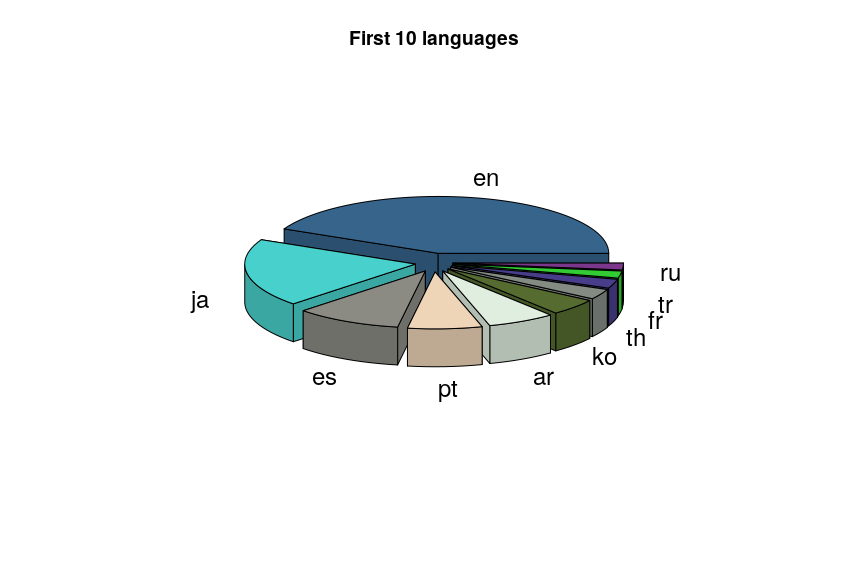
\includegraphics[width=\linewidth]{first_ten_languages.png}}
\caption{Results for 1 208 516 638 tweets analysed (deleted tweet was not count)}
  \label{fig:trump_results}
\end{figure}


\subsection{Pre-Processing}
\label{subsub:preprocessing}

In this paper we introduce two new resources for pre-processing twitter data \cite{Jianqiang17}, we used some of their ideas like removing URL, as you can see in the repository, an emoticon dictionary is available in Python and we can remove them from any tweets.Some labe were considered irrelevant \cite{Poddar16} because we think that it is more relevant to detect bots and not adding them into the analyse process rather than put a tag on them and lose time of computation for sentiment analysis. It is powerful because even it is relevant, we can’t take them for computing them after due to a problem of time. Positive, Negative, and Neutral are the three labels for Sentiment Analysis and Joy, Fear, Anger, Surprise and Sadness are the fifth labels for Emotion Analysis. We pre-process all the tweets as follows:
\begin{itemize}
\item  We remove all the emoticons.
\item  We remove all URLs with a regular expression. 
\item  Replace targets (e.g. “@John”) by also removing them.
\item  Removing "RT" for most of the tweets, because it doesn't mean something for the application. 
\end{itemize}
Tweets in a general way contain a lot of opinions but they are expressed in different ways by users, as they did \cite{Rebecca11} by keeping emoticons. It deals with the preparation that removes the repeated words and punctuations and improves the efficiency the data. Forward other process is doing like converting upper case to lower case. User names and URLs are not important from the perspective of future processing so their presence is irrelevant. All usernames and URLs are removed to improve the real result. 


\subsection{Machine learning for Emotion and Sentiment classification}
\label{subsub:ml}

In order to predict the feeling (Postive, negative, neutral) and emotion (joy, anger, sadness, fear, surprise) for each tweet, we used 2 methods. They used other label for emotions that we did not to determine the feeling of the tweet, we used the TextBlob librairy which provides a simple API of Natural Languge processing and thus allows us to make the sentiment analysis. For this, TextBloB calculates a Polarity rate of -1 to +1 or -1 corresponds to an extremely negative twitch and an extremely positive +1.
To determine the emotion, we had to create our own classification model (classification in English what) with scikit-learn.
To do this we took a tweet dataset that we labalised (after having data cleaned as indicated in the previous paragraph) thanks to Indico, an enterprise AI solution for unstructured content. Their focus is on helping to automate tedious back-office tasks, improving the efficiency of labor-intensive document-based workflows, and extracting valuable insights from your unstructured content, including text and images.  
We then transform this dataset into a term document matrix and apply a TF-IDF standardization to evaluate the importance of the term content in each tweet.
Finally, we applied a SVM for the classification because like they said \cite{Medhat14}, it is very suitable for text data.
Once the model was extracted, we used it with Spark to predict the emotion of all tweets.

\subsection{Feature Generation}
\label{subsub:featureGeneration}

Take the example of a two-step algorithm, MapReduce will have to perform two jobs:
At the first job:
\begin{enumerate}
\item	Read the initial data.
\item	Execute step 1 in a first job.
\item	Save the intermediate result in a distributed way.
\end{enumerate}
In the second job:
\begin{enumerate}
\item	Read this result.
\item	Execute step 2.
\item	Save the result in a distributed way.
\end{enumerate}
Spark shares the RDD (Resilient Distributed Datasets) with the initial data and, by applying step 1, will provide in step 2 a "virtual" intermediate RDD representing the result of step 1 without necessarily immediately rotating the calculation. When the result of step 2 is requested, Spark will combine the calculations required in steps 1 and 2 into one Spark job that will:
\begin{enumerate}
\item	Read the initial data.
\item	Perform steps 1 and 2, the intermediate result remaining in memory.
\item	Save the result in a distributed way.
\end{enumerate}
Spark thus avoids expensive distributed writing and replay and then only requires the execution of one job (each job having an incompressible structure cost).
When the algorithm has several steps, the time saving becomes considerable!
Two types of operations (In technical terms, Spark calculates a direct acyclic graph of the operations to be performed, like Apache Storm or Apache Tez) can be performed on RDDs: transformations and actions. Transformations return a new "virtual" RDD: nothing is then evaluated or persisted, while the actions evaluate and return a value. After an action, all the previous transformations are then computed (see the repository in the compute folder).

\section{Deep Learning}
\label{sec:dp}
\href{http://tex.stackexchange.com}{This is a very very
  very very very very very very very very very very very very very
  very very very very very very very very long link.}
\subsection{Data Processing and Architecture}
\label{subsub:dl}

First, we downloaded the dataset of 1 578 627 tweets pre-classified, then we read the dataset from the CSV into two files (.pos and .ned) with (see csv\_parser.py). Then we generate a CSV with the vocabulary (and its inverse mapping) with an another process. Each vocabulary has a weight.
For example if a name is wrote, we remplace it by \textless 
NAME/\textgreater and the same thing for a link : \textless LINK/\textgreater.
The network implemented in this script is a single layer CNN (Convolutional Neural Networks)  structured as follows:
\begin{itemize}
\item  \textbf{Embedding layer}: takes as input the tweets (as strings) and maps each word to an n-dimensional space so that it is represented as a sparse vector (see word2vec).
\item  \textbf{Convolution layers}: a set of parallel 1D convolutional layers with the given filter sizes and 128 output channels. A filter's size is the number of embedded words that the filter covers.
\item  \textbf{Pooling layers}: a set of pooling layers associated to each of the convolutional layers.
\item  \textbf{Concat layer}: concatenates the output of the different pooling layers into a single tensor.
\item  \textbf{Dropout layer}: performs neuron dropout (some neurons are randomly not considered during training).
\item  \textbf{Output layer}: fully connected layer with a softmax activation function to perform classification.
\end{itemize}

\subsection{TensorFlow}
\label{subsub:dl}

TensorFlow is an open source machine learning tool developed by Google. The source code was opened on November 9, 2015 by Google and released under Apache license.
It is based on the DistBelief infrastructure, initiated by Google in 2011, and is equipped with a Python interface.
TensorFlow is one of the most used tools in AI in the field of machine learning and deep learning.
We used an architecture based on previous work (here)\footnote{\url{https://github.com/danielegrattarola/twitter-sentiment-cnn}}.
Even we used a GTX 1060 (1212 cuda cores compared to the Titan V which was developed for Deep Learning with 5120 cuda core), it took around 2h20 to train the CNN.
The course of the exection is available in the file "log.log".
The neural network weighs about 424.1 MB.
You can download in JSON or CSV format the results for the validation of the training loss here\footnote{\url{https://github.com/mbenhamd/twitter-sentiment-cnn}}.

The graphics below can be found thanks to the TensorFlow web interface.
To summarize 110 990 iterations, 10 epochs, validation accuracy: 0.825287, loss of training: 49.6865

\begin{figure}[H]
{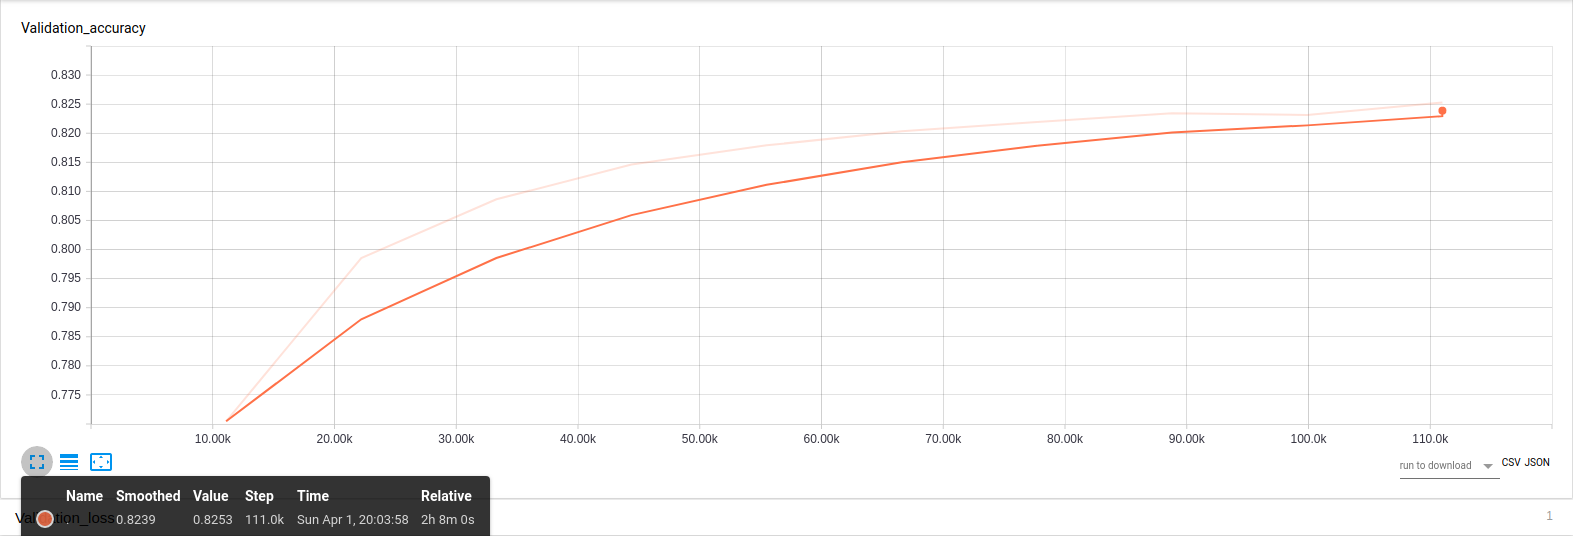
\includegraphics[width=\linewidth]{validation-accuracy.png}}
\caption{Schema of Validation Accuracy From TensorFlow Interface Web.}
  \label{fig:archivedb}
\end{figure}

We can see a logarithmic evolution of the accuracy of the neuron network, 82\% is in itself a low result in the sense that neural networks methods are expected to be accurate to 95\% minimum in practical cases. For the text classification case, the dataset of tweets do not contain enough vocabulary to allow us a large-scale use.

\begin{figure}[H]
{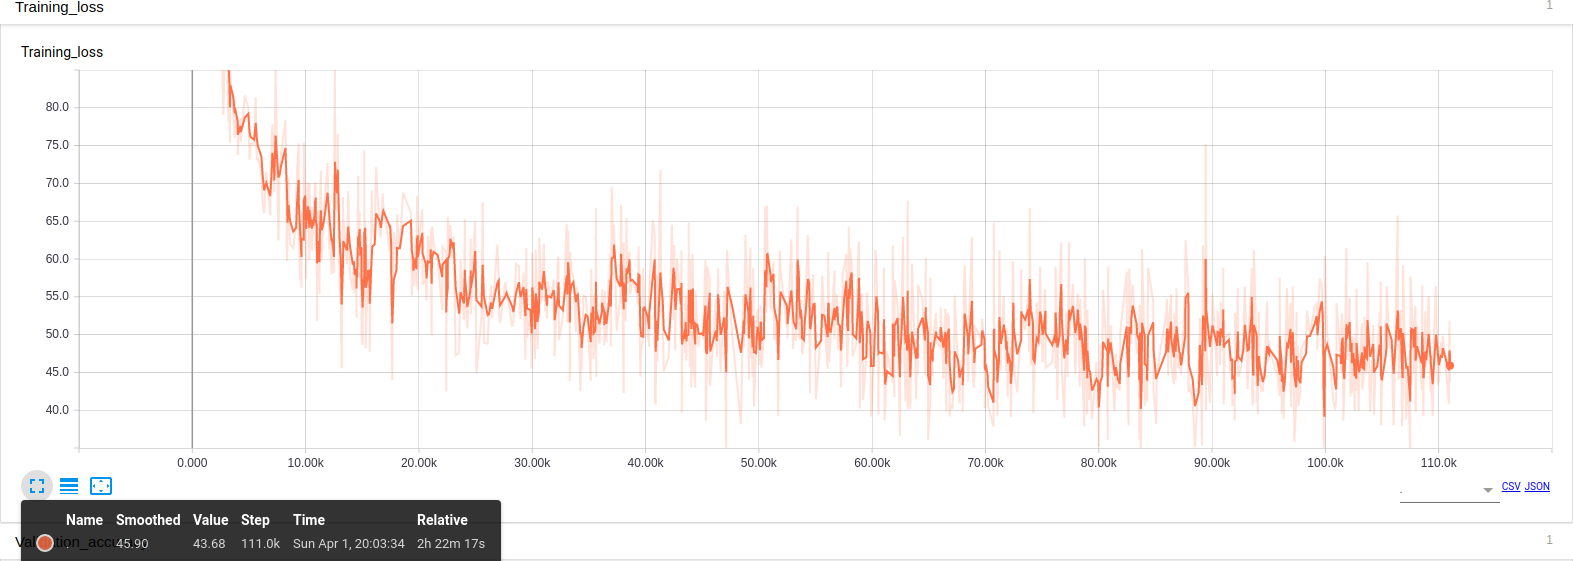
\includegraphics[width=\linewidth]{training-loss.png}}
\caption{Schema of Training Loss From TensorFlow Interface Web.}
  \label{fig:archivedb}
\end{figure}


The validation loss here is 49.68 and the lower the loss, the better model (unless the model has over-fitted to the training data). The loss is calculated on training and validation and its interperation is how well the model is doing for these two sets. Unlike accuracy, loss is not a percentage. It is a summation of the errors made for example in training or validation sets.
In the case of neural networks, the loss is usually negative log-likelihood and residual sum of squares for classification and regression respectively. Then naturally, the main objective in a learning model is to reduce the value of the loss of the value of the product.
Loss value implies a certain model behaves after each iteration of optimization. Ideally, one would expect the reduction of loss after each, or several iterations.
The accuracy of a model is usually determined by the model parameters and is determined. Then the test samples are fed to the model and the number of mistakes (zero-one loss) the model is recorded, after comparison to the true targets. Then the percentage of misclassification is calculated.
For example, if the number of test samples is 1000 and model classifies 952 of those correctly, then the model's accuracy is 95.2\%.
Here is a summary of training loss and validation accuracy (done with Spark with the describe function).


\begin{table}[H]
\tbl{Training Loss describe}{%
\begin{tabular}[width=\linewidth]{rcrcrcrc@{0.5in}}
Summary & {Wall Time} & {Step} & {Value} \\
$Mean$ & \[1.59x10^9\] & 552 51.293 & 56.1645 \\
$Stddev$ & 2470.404 & 32 058.352 & 22.553 \\
$Min$ & \[1.52x10^9\] & 100 157 & 102.860 \\
$Max$ & \[1.52x10^9\] & 99 954 & 97.983 \\
\end{tabular}}
\label{tab:training_loss_a}
\end{table}


\begin{table}[H]
\tbl{Validation Accuracy Describe}{%
\begin{tabular}[width=\linewidth]{rcrcrcrc@{0.5in}}
Summary &{Wall Time} &{Step} &{Value} \\
$Mean$ & \[1.59x10^9\] & 65585.818 & 0.81360 \\
$Stddev$ & 2701.1972 & 35258.454 & 0.01645 \\
$Min$ & \[1.52x10^9\] & 11 099 & 0.7704 \\
$Max$ & \[1.52x10^9\] & 99 891 & 0.8252 \\
\end{tabular}}
\label{tab:valid_loss_b}
\end{table}

To conclude, as you can see, the previous work had a final validation accuracy of 0.80976, and a validation loss of 53.3314, as the author wrote in GitHub. We download the model and checked the summaries via tensorboard an we saw that the model shared took around 4h13 to train with 33 297 iterations (3 epochs), the validation accuracy was 0.80976 and validation loss was 53.3314.

\section{Implementation}
\label{sec:implementation}

We have used the following technologies for many reasons. Hadoop assumes that conventional approaches (consisting of developing ever more powerful centralized systems) have technical and financial limitations. The development of distributed systems consisting of machines or nodes, relatively affordable (commodity hardware) and scaling out is an alternative from a technical and financial point of view because a distributed system comprising tens, hundreds or thousands of nodes will regularly be confronted with hardware and/or software failures. Google has developed the Google File System (GFS), ancestor of the Hadoop Disrelated File System (HDFS) \cite{Baltas17} and the MapReduce Approach.Hadoop is particularly effective for dealing with problems that have one or more of the following characteristics: Volume of data to store or process very important. Need to perform processing on all data (batch rather than transactional, therefore). Heterogeneous data in terms of origin, structure, and format (JSON for example, Tweets collected via any Tweeter API are send in JSON because of the flexibility of this type of object. Several examples are in the repository for interested readers). Execute the tasks of an Hadoop job in parallel, without a pre-established order. An Hadoop cluster is made up of tens, hundreds, or thousands of nodes. It is the addition of the storage and processing capacities of each of these nodes which makes it possible to offer a storage space and a computing power yet to handle data volumes of several To or Po. To improve the performance, Hadoop's file management system, HDFS, writes and reads files in blocks of 64 MB or 128 MB. Working on such large blocks maximizes data transfer rates by limiting search time on hard drives (seek time). MapReduce is a programming model designed specifically to read, process and write very large volumes of data. An Hadoop program usually implements both map and reduce tasks, those programs are usually divided into three parts: The driver, which runs on a client machine, is responsible for configuring the job and submitting it for execution. The map is responsible for reading and processing data stored on disk. The reducer is responsible for consolidating the results from the map and write them on disk. Naturally, the implementation core use Hadoop for those reasons.

\section{Web application}
\label{sec:web_application}


\subsection{Conception of the DataBase (Web Site)}
\label{subsub:conception_db}

In order to allow quick access to the data on the website at any time, we could use technologies from AWS but finally, by budget limitation, we can not offer a database with a very strong capacity of CPU or datawharehouse we can manage PB of data. The PostgresSQL database is based on a micro instance of 1 CPU and 2 GB of RAM.
With this configuration, it is clearly impossible to perform complicated SQL Queries such as group by, and other aggregation on 350 millions lines.
For this reason, we decided to optimize our database and create a table corresponding to a data item that we want to display. The query is thus done only on indexes, the response time is then very fast (100ms maximum) regardless of the size of the table.
To do this, we had to proceed by step severals steps.
The first step was to define exactly the data we wanted to display: We selected temporal data (Psychological evolution during the year, for each month, according to the time), as well as trends, better users and best retweets monthly / yearly. We also chose to be able to display the psychological profile for each user (Global psychological evaluation, number of tweet / retweet and evolution over the year).
Then the second step, we coded Spark scripts for each problem to calculate what we wanted to display. All calculation scripts are here\footnote{\url{https://github.com/yannistannier/twitter-sentiment-analysis/tree/master/compute}}. 
To finish, the third step, each Spark script returned us an aggregated file as we wanted, we just had to import these files into the corresponding tables taking care to organize our indexes.
For example: to retrieve the psychological evolution of a user, we just have to make a simple SQL Query on the table {\itshape user\_stat} with a selection on index (where id = 1656561) and the query we reference in 100ms, 12 rows corresponding to each month. The same request with several accreditation operators on the initial table took several minutes to answer us.


\begin{figure}[H]
{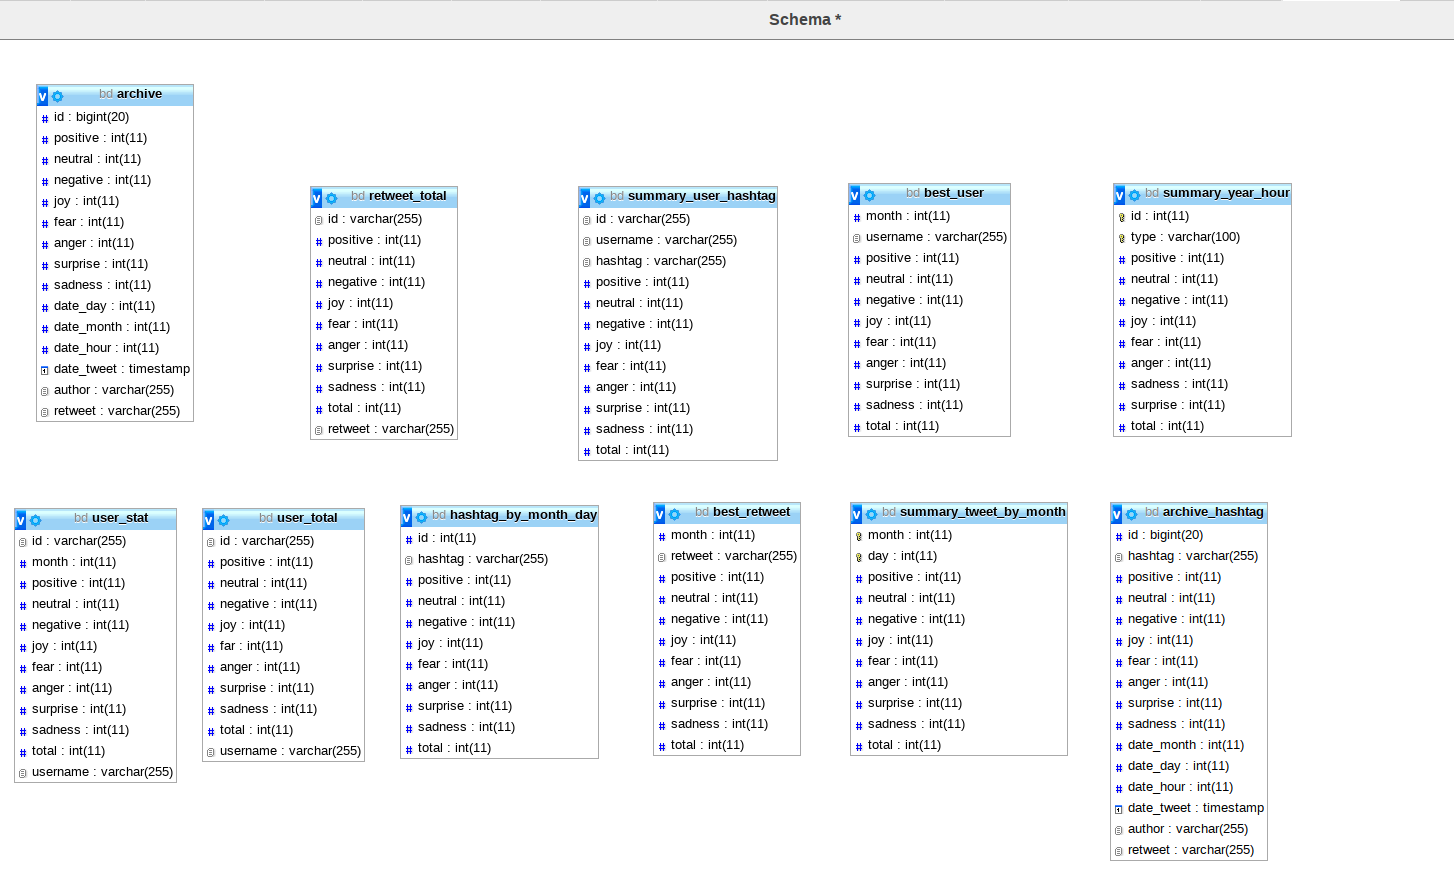
\includegraphics[width=\linewidth]{table-web-db.png}}
\caption{Schema of the DataBase.}
  \label{fig:archivedb}
\end{figure}


\subsection{Conception of the Archive Access}
\label{subsub:conception_aa}

Once the database was created, we wanted the render very easily accessible to the public and we have developed a web platform.
The platform presents a very classic web architecture. Our database PostgresSQL with aggreger data is hosted by AWS RDS.
We have developed an API Rest through AWS Lambda and AWS GateWey that are responsible for executing SQL requests and returning formatting data.
And finally our web client React.js which his role is to call the API Rest and display data.

\subsection{Conception of the Real Stream}
\label{subsub:conception_rs}

For the real-time part, we chose to use Kinesis Data Streams, which is the real-time data analysis service of AWS.
For this we have created a Tweet Streamer that is responsible for recovering real-time data via the API Stream of twitter. This data is sent to Kinesis Data Streams which allows you to aggregate data from multiple sources.
Those data are thus sent to a consumer who is responsible for analyzing and predicting emotions and feelings in real time through TextBloB and our model of emotion prediction.
Once the data is analyzed, our Consumer formats them and sends the result to our web client thanks to MQTT.
Real-time streams scripts can be found here\footnote{\url{https://github.com/yannistannier/twitter-sentiment-analysis/tree/master/kinesis-realtime}}.
The streamTwitter.py file is our Twitter streamer and the kinesisStream.py file is our Consumer.


\begin{figure}[H]
{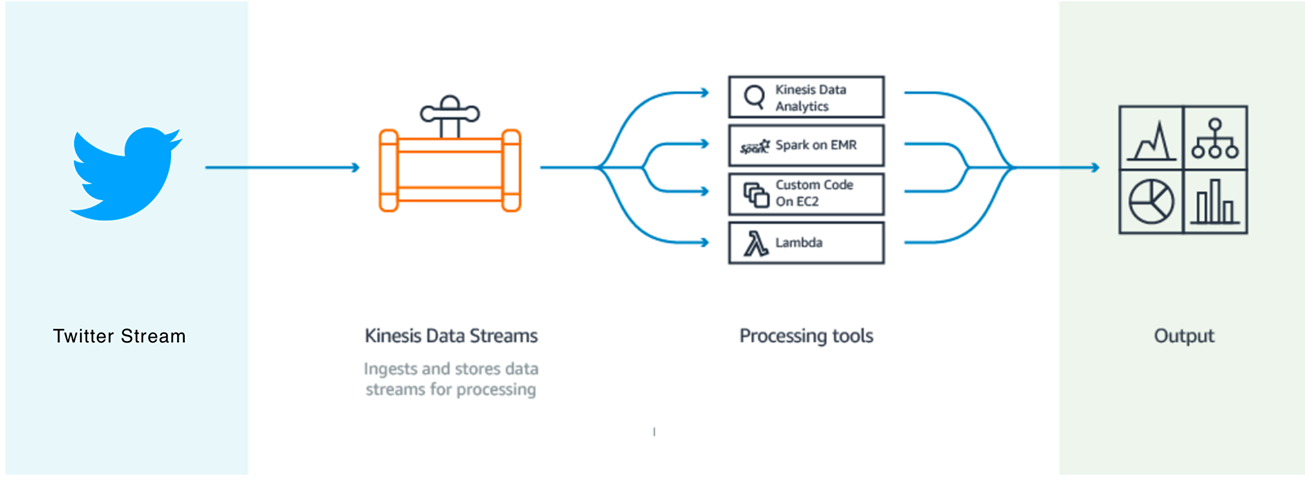
\includegraphics[width=\linewidth]{real_stream-schema.png}}
\caption{Schema for the Real Stream Web Application.}
  \label{fig:archivers}
\end{figure}

\section{Results}
\label{sub:results}

\subsection{Classification - F-Measure}
\label{subsub:english_tweets_monthly}

\begin{table}[H]
\tbl{Binary Classification Results}{%
\begin{tabular}[width=\linewidth]{rcrcrc@{0.5in}}
Classifier &{Best Solution Publication} &{Our Solution}  \\
$Naives Bayes$ &  0.728 & 0.772 \\
$Logistic Regression$ & 0.665 & 0.78 \\
$Decision Trees$ &  0.597 & 0.68 \\
$Random Forest$ &  - & 0.72 \\
$Linear SVM$ &  - & 0.80 \\
$SGB Classifier$ & - & 0.74 \\
\end{tabular}}
\label{tab:binary}
\end{table}

\begin{table}[H]
\tbl{Ternary Classification Results From Publication}{%
\begin{tabular}[width=\linewidth]{rcrcrcrcrc@{0.5in}}
Classifier &{Positive} &{Negative} &{Neutral} &{Total}  \\
$Naives Bayes$ &  0.717 & 0.75 & 0.617 & 0.696 \\
$Logistic Regression$ & 0.628 & 0.592 & 0.542 & 0.591 \\
$Decision Trees$ &  0.646 & 0.727 & 0.557 & 0.643 \\
\end{tabular}}
\label{tab:binary}
\end{table}

\begin{table}[H]
\tbl{Our Results For Ternary Classification Results}{%
\begin{tabular}[width=\linewidth]{rcrcrcrcrc@{0.5in}}
Classifier &{Positive} &{Negative} &{Neutral} &{Total}  \\
$Naives Bayes$ &  0.54 & 0.72 & 0.60 & 0.63 \\
$Logistic Regression$ & 0.62 & 0.74 & 0.64 & 0.67 \\
$Decision Trees$ &  0.58 & 0.68 & 0.59 & 0.62 \\
$Random Forest$ &  0.58 & 0.72 & 0.62 & 0.65 \\
$Linear SVM$ &  0.61 & 0.72 & 0.62 & 0.66 \\
$SGB Classifier$ &  0.60 & 0.74 & 0.62 & 0.66 \\
\end{tabular}}
\label{tab:binary}
\end{table}

As we early introduced in related work, we can say that in the case of the binary classification, our method of pre-processing the data gives better results than others.
We can also see that the SVM allows us to have the best accuracy.
However, in the case of ternary classification, the method of publication is superior.

\subsection{English tweets monthly analyzed}
\label{subsub:english_tweets_monthly}

We analyzed the set of English tweets on the year, dividing by month to see any evolution or regression during the year. A thorough American sociological study on the year 2017 could give the reasons for the graph. We were surprised at the symmetry between joy and sadness, proof that the emotional analysis is not as biased as one might think. 

\begin{figure}[H]
{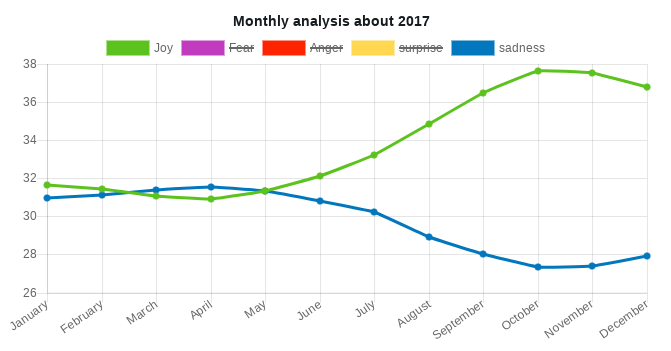
\includegraphics[width=\linewidth]{monthly_analysis_joy_sadness-exemple.png}}
\caption{Results by month for joy and sadness emotions during the 2017.}
  \label{fig:trump_results}
\end{figure}

\subsection{Psychological profile for any users}
\label{subsub:psychological_profile}

We have implemented a psychological profile by current user in the database (note that this feature and also available in the case of streaming too).Structure similarity context are also in search \cite{Zou18}.The problem of sentiment analysis from archive tweets is that there are not so many tweets for each user as we imagine so we have a lack of data problem.
We implemented a solution in the website \footnote{\url{https://twitter.yannistannier.io/#/archive/user}}.

\subsection{Impacts of tweets}
\label{subsub:impacts_tweets}

In this section, we wanted to talk about the effect of tweets on the community, taking one of the most retweeted user, Donald Trump. We have 414 716 retweet which allows to have a number of acceptable messages to use the word "impacts". In this publication, \cite{Vyas17}, we found interisting their fought on what they call "influence" and tools used about that. It is interesting in the field of politics but also in the media world to have an analysis of what is said and done in the world today.

\begin{figure}[H]
{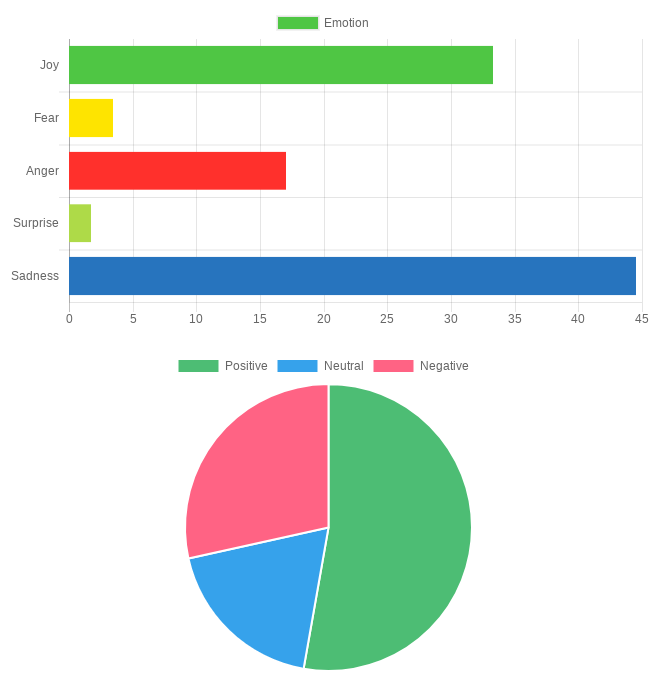
\includegraphics[width=\linewidth]{retweeted_emotion_sentiment_trump-exemple.png}}
\caption{Results for the emotions ratio on the 414 716 retweeted Donald Trump tweets computed.}
  \label{fig:trump_results}
\end{figure}

\subsection{English tweets monthly analyzed}
\label{subsub:english_tweets_monthly}

We analyzed the set of English tweets on the year, dividing by month to see any evolution or regression during the year. A thorough American sociological study on the year 2017 could give the reasons for the graph. We were surprised at the symmetry between joy and sadness, proof that the emotional analysis is not as biased as one might think. 

\subsection{Comparaison of TextBloB and True Results for Emotion Relation}
\label{subsub:comparaisonEmotionRelation}

We will now discuss the consistency of results.

\begin{figure}[h!]
{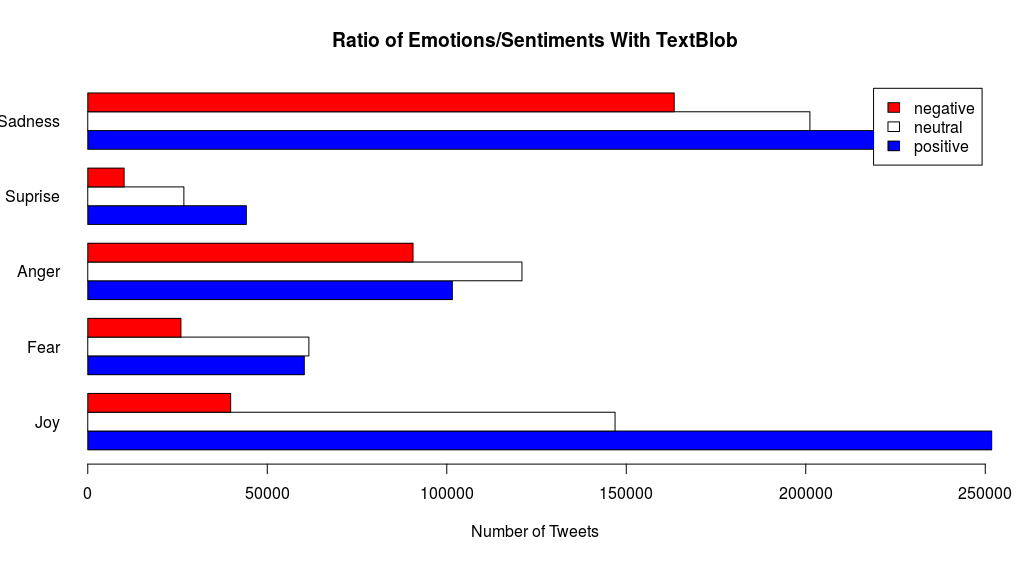
\includegraphics[width=\linewidth]{ratio-textblob.png}}
\caption{Results for ratio Emotion/Sentiment with Number of tweets using TextBlob}
  \label{fig:contradiction_barplot}
\end{figure}

In this paragraph we will start with TextBloB, the famous sentiment analyzer in the world of open source. The problem here is that the library offers 3 variables for feelings. We can see that tweets are considered either negative, positive, or neutral gold in the basic data set we only have 2 possible values ​​(positive or negative). Here there is a contradiction of analysis, the sad messages are mostly positive. The explanation here is that a number of tweet considered neutral should be either positive or negative, the introduction of this new posibility of values ​​makes the model over-learning (it's not a over-fitting problem) for feelings. Below is a summary table with the exact values.

\begin{table}[H]
\tbl{Cross Tab between sentiments and emotions using TextBloB}{%
\begin{tabular}[width=\linewidth]{rcrcrcrcrcrc@{0.5in}}
S\textbackslash E &{Joy} &{Fear} &{Anger} &{Surprise} &{Sadness} \\
$Positive$ & 251 787 & 60 325 & 101 556 & 441 75 & 233 604  \\
$Neutral$ & 146 876 & 61 592 & 120 944 & 26 772 & 201154 \\
$Negative$ & 39 802 & 25 950 & 90 601 & 10 131 & 163 358 \\
\end{tabular}}
\label{tab:cross_tab_TextBLOB}
\end{table}


We do not have emotions variables in order to have an overview of our model of emotions to train from an SVM but as this graph indicates, there is a coherence in our results. Sad messages are considered negative and happy messages are positive. For the other cases, it would be necessary to realize a psychological study between feelings and emotions in oneself.

\begin{figure}[h!]
{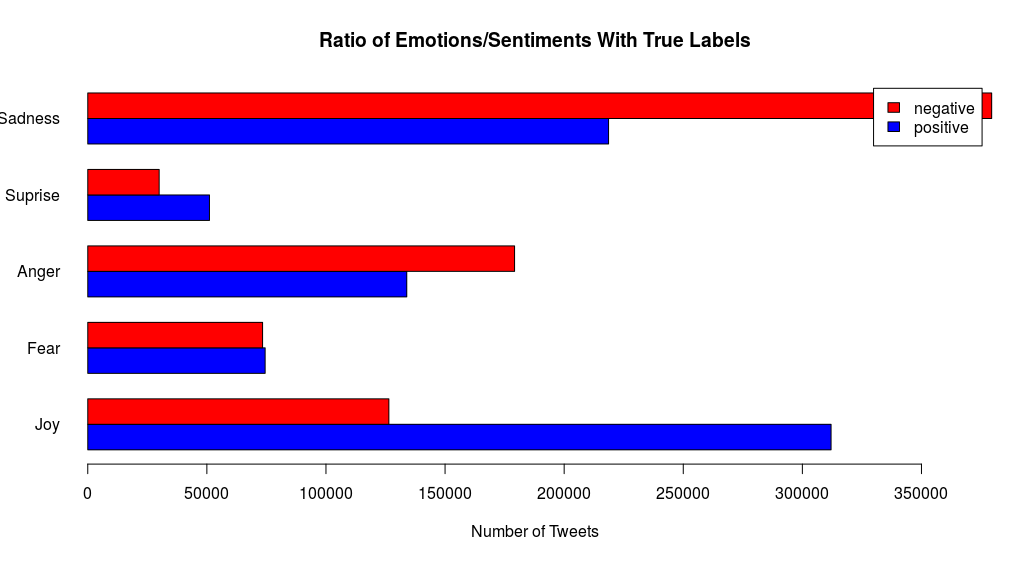
\includegraphics[width=\linewidth]{ratio-true-labels.png}}
\caption{Results for ratio Emotion/Sentiment with Number of tweets using True Labels}
  \label{fig:contradiction_barplot}
\end{figure}

\begin{table}[H]
\tbl{Cross Tab between sentiments and emotions using True Labels}{%
\begin{tabular}[width=\linewidth]{rcrcrcrcrcrc@{0.5in}}
S\textbackslash E &{Joy} &{Fear} &{Anger} &{Surprise} &{Sadness} \\
$Positive$ & 312 055 & 74 474 & 133 921 & 51 094 & 218 641  \\
$Negative$ & 126 410 & 73 393 & 179 180 & 29 984 & 379 475 \\
\end{tabular}}
\label{tab:cross_tab_TrueLabels}
\end{table}

Above the results obtained for the list of tweets that are 1,578,627 in the sample.

\section{Discussion}
\label{sec:discussion}

We now turn our attention to the following interesting question: whether the subjective data that exist on the web carry useful information. This is an example with a sample of 383 623 424 tweets in English.

\begin{table}[H]
\tbl{Cross Tab between sentiments and emotions}{%
\begin{tabular}[width=\linewidth]{rcrcrcrcrcrc@{0.5in}}
S\textbackslash E &{Joy} &{Fear} &{Anger} &{Surprise} &{Sadness} \\
$Positive$ & 63 559 579 & 9 296 846 & 27 861 247 & 7 768 707 & 42 382 993  \\
$Neutral$ & 55 127 659 & 15 777 833 & 42 460 015 & 8 879 626 & 48 232 835 \\
$Negative$ & 9 054 496 & 3 395 622 & 23 281 712 & 1 948 578 & 24 595 676 \\
\end{tabular}}
\label{tab:cross_tab}
\end{table}

According to this view, the diversity and pluralism of information on different topics can have negative role. It is well understood, that true knowledge is being described by facts, rather than subjective opinions \cite{ThakkarP15}. However, this diversity in opinions, when analyzed, may deliver new information and contribute to the overall knowledge of a subject matter. This is especially true when the object of our study is the attitude of people. In this case, opinion native data can be useful to uncover the distribution of sentiments across time, or different groups of people. However, data mining differs from machine learning and statistics in that it deals with large volumes of data, stored primarily on disk. Some types of knowledge discovered from a database can be represented by a set of rules. The following is an example of a rule, stated informally: “Donald Trump and his totals of retweets incomes are greater than the average with the most sadly effects on users”. Of course, such riles are not universally true, and have degrees of "support" and "confidence". Other types of knowledge are represented by equations relating different variables to each other, or by other mechanisms for predicting outcomes when the values of some variables are known. There are a variety of possible types of patterns that may be useful, and different techniques are used to find different types of patterns. Usually there is a manual component to data mining, consisting of preprocessing data to a form acceptable to the algorithms and post-processing of discovered patterns. For this reason, data mining is really a semiautomatic process in real life. The mode widely used applications are those that requires some sort of prediction. In our case, we want to predict emotions and sentiments, then a psychological profile. Abstractly, the classification problem is this: Given that user in the archive, and given his tweet. We use a given instances of items along with the classes to which they belong, the problem is to predict the class. Since we associate several classes together, then we come to conflicting analyzes. 

\begin{figure}[h!]
{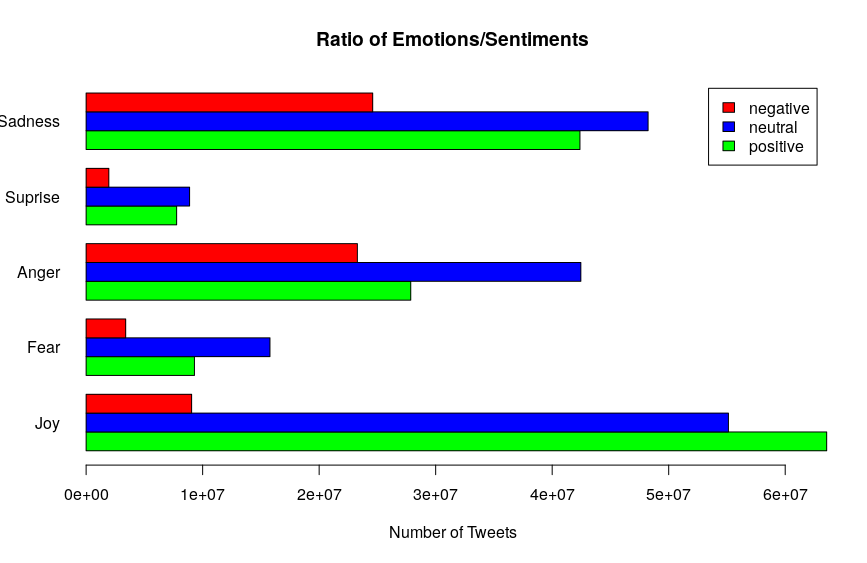
\includegraphics[width=\linewidth]{final_plot_contradiction_analysis.png}}
\caption{Results for ratio Emotion/Sentiment with Number of tweets}
  \label{fig:contradiction_barplot}
\end{figure}

First non-surprising results like Joy/Positive at 49.75 \% and Joy/Negative at 7.08 \%.
We can see that we normally associate sadness with something negative, but here we see that positive feelings are predominant, just as anger has a majority of positive feelings. One publication can also be referred \cite{Alm05} because accordly to this addition between emotion and sentiment, they also have other results.

\section{Conclusion and Future Work}
\label{sec:conclusion}

In this report we have presented a sentiment analysis tool on a Web interface. In one hand we used data from an archive and in the other hand we used real time stream analysis. Due to the absence of labelled data we couldn't argue on reliability of data.  This recent publication really question us about the limit on software engineering \cite{Lin18}, but they did not explored deep learning \cite{Meisheri17} and what we could achieve with this learning techniques using neural network fully connected that we always only get better with time because of optimized function behind and great computation that we have due to GPU in aim to build deep learning classifier \cite{Araque17}. 
There are also other features for the real stream \footnote{\url{https://twitter.yannistannier.io/#/realtime}} such as geolocation of people, we could then generate a graph as a center to any user and know its impact on an interactive map, this would allow among other things to know the influence for example. To conclude, we think that having access to geolocation data and build a powerful neural network trained and design for sentiment analysis could be a great idea for future work. 

\section{References}

\begin{acks}
We are grateful to the following people for resources, discussions and suggestions: Jason Scott (Archivist) for his website and allowing people to get some data useful for research and other things. We also wanted to thanks Diana Yuan (Co-Founder & Vice President, Talent & Operations from Indico), we exchanged a lot of emails and she agreed to increase the numbers of calls from their API freely (initially it is 10 000 calls per day).
\end{acks}

% Bibliography

\bibliographystyle{ACM-Reference-Format-Journals}
\bibliography{publication-bibfile}

\end{document}
